\section{Casos de uso}

\begin{figure}[H]
  \centering
  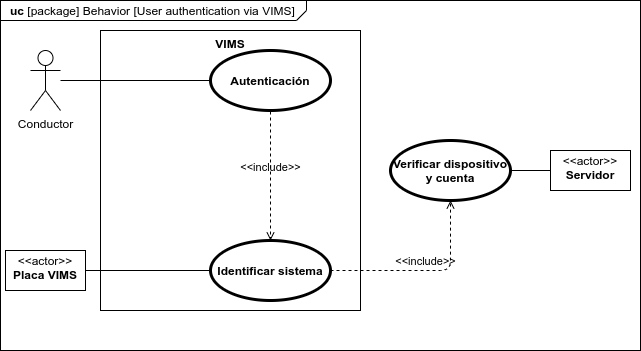
\includegraphics[width=\linewidth]{diagrams/UseCases-UC1 - auth.png}
  \caption{Caso de uso \texttt{01} -- \textit{autenticación}.}
  \label{uc:auth}
\end{figure}

\begin{table}[H]
  \centering
  \begin{tabularx}{\textwidth}{|c|c|X|}
    \hline
    \texttt{01}                                & \multicolumn{2}{c|}{\textit{Autenticación}}                                                                                                                                                                                                                 \\
    \hline
    \textbf{Descripción}                       & \multicolumn{2}{X|}{La placa identificará de forma inequívoca al conductor (usuario) y a sí misma frente al servidor.}                                                                                                                                      \\
    \hline
    \multirow{9}{*}{\textbf{Secuencia normal}} & \textbf{Paso}                                                                                                          & \textbf{Acción}                                                                                                                    \\
    \cline{2-3}
                                               & 1                                                                                                                      & \multicolumn{1}{L|}{El usuario se autentica contra la placa con su cuenta personal ya creada.}                                     \\
    \cline{2-3}
                                               & 2                                                                                                                      & \multicolumn{1}{L|}{La placa \ac{VIMS} recoge la información del usuario y la envía al servidor junto con su identificador único.} \\
    \cline{2-3}
                                               & 3                                                                                                                      & \multicolumn{1}{L|}{El servidor verifica que la cuenta del usuario existe y se asocia la información al dispositivo.}              \\
    \cline{2-3}
                                               & 4                                                                                                                      & \multicolumn{1}{L|}{La placa almacena la información del usuario y finaliza el proceso de inicio de sesión.}                       \\
    \hline
    \multirow{4}{*}{\textbf{Excepciones}}      & \textbf{Paso}                                                                                                          & \textbf{Acción}                                                                                                                    \\
    \cline{2-3}
                                               & 2                                                                                                                      & \multicolumn{1}{L|}{La placa no cuenta con conexión a la red o el servidor no está disponible.}                                    \\
    \cline{2-3}
                                               & 3                                                                                                                      & \multicolumn{1}{L|}{La cuenta del usuario no existe.}                                                                              \\
    \hline\hline
    \textbf{Resolución}                        & \multicolumn{2}{X|}{La placa funciona en modo desconectado, es decir, no transmite datos al servidor.}                                                                                                                                                      \\
    \hline
  \end{tabularx}
\end{table}

\noindent\rule{\linewidth}{.2pt}

\begin{figure}[H]
  \centering
  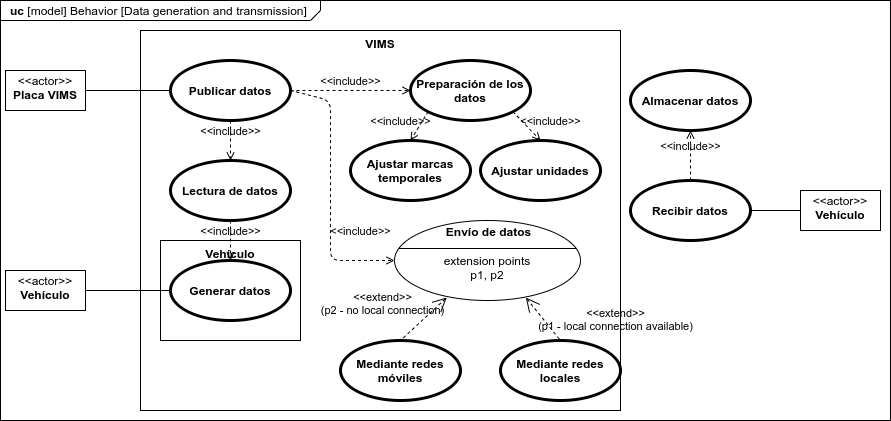
\includegraphics[width=\linewidth]{diagrams/UseCases-UC2 - data.png}
  \caption{Casos de uso \texttt{02} -- \textit{generación y transmisión de datos}.}
  \label{uc:data}
\end{figure}

\begin{table}[H]
  \centering
  \begin{tabularx}{\textwidth}{|c|c|X|}
    \hline
    \texttt{02}                                 & \multicolumn{2}{c|}{\textit{Generación y transmisión de datos}}                                                                                                                                                                                                                                                                                                                             \\
    \hline
    \textbf{Descripción}                        & \multicolumn{2}{X|}{El dispositivo \ac{VIMS} recibirá los datos del vehículo al que está conectado y los preparará para una posterior transmisión al servidor remoto de almacenamiento y gestión.}                                                                                                                                                                                          \\
    \hline
    \multirow{10}{*}{\textbf{Secuencia normal}} & \textbf{Paso}                                                                                                                                                                                                                & \textbf{Acción}                                                                                                                                              \\
    \cline{2-3}
                                                & 1                                                                                                                                                                                                                            & \multicolumn{1}{L|}{La placa \ac{VIMS} recibe los datos que el vehículo está generando de forma continuada.}                                                 \\
    \cline{2-3}
                                                & 2                                                                                                                                                                                                                            & \multicolumn{1}{L|}{Los datos recibidos se preparan para el envío, ajustando cierta información y añadiendo valores como la cuenta asociada a dichos datos.} \\
    \cline{2-3}
                                                & 3                                                                                                                                                                                                                            & \multicolumn{1}{L|}{Mediante el uso de redes móviles o locales, según disponibilidad, se envían los datos al servidor.}                                      \\
    \cline{2-3}
                                                & 4                                                                                                                                                                                                                            & \multicolumn{1}{L|}{El servidor recibe la información transmitida por el sistema y la almacena para una posterior visualización y tratamiento.}              \\
    \hline
    \multirow{9}{*}{\textbf{Excepciones}}       & \textbf{Paso}                                                                                                                                                                                                                & \textbf{Acción}                                                                                                                                              \\
    \cline{2-3}
                                                & 1                                                                                                                                                                                                                            & \multicolumn{1}{L|}{El vehículo no está conectado o no transmite datos.}                                                                                     \\
    \cline{2-3}
                                                & 2                                                                                                                                                                                                                            & \multicolumn{1}{L|}{Todavía no hay ninguna cuenta asociada a la placa \ac{VIMS}.}                                                                            \\
    \cline{2-3}
                                                & 3.1                                                                                                                                                                                                                          & \multicolumn{1}{L|}{No hay redes móviles disponibles, se intenta transmitir por redes locales.}                                                              \\
    \cline{2-3}
                                                & 3.2                                                                                                                                                                                                                          & \multicolumn{1}{L|}{No hay redes locales disponibles, se intenta transmitir por redes móviles.}                                                              \\
    \cline{2-3}
                                                & 3.3                                                                                                                                                                                                                          & \multicolumn{1}{L|}{No hay redes disponibles, se almacenan los datos para su posterior transmisión.}                                                         \\
    \hline\hline
    \textbf{Resolución}                         & \multicolumn{2}{X|}{La placa funciona en modo desconectado, es decir, no transmite datos al servidor. Si existe una cuenta asociada pero no hay conexión, los datos se almacenan en memoria hasta que se puedan transmitir.}                                                                                                                                                                \\
    \hline
  \end{tabularx}
\end{table}

\noindent\rule{\linewidth}{.2pt}

\begin{figure}[H]
  \centering
  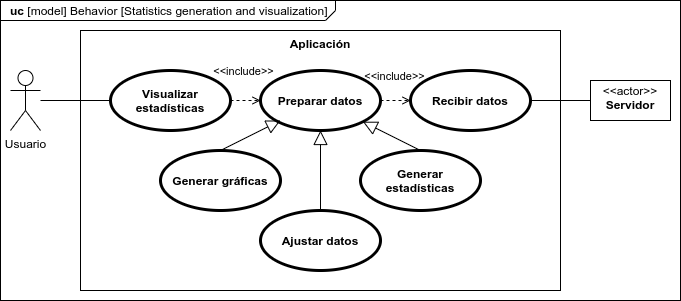
\includegraphics[width=\linewidth]{diagrams/UseCases-UC3 - stats.png}
  \caption{Caso de uso \texttt{03} -- \textit{generación de estadísticas}.}
  \label{uc:stats}
\end{figure}

\begin{table}[H]
  \centering
  \begin{tabularx}{\textwidth}{|c|c|X|}
    \hline
    \texttt{03}                                & \multicolumn{2}{c|}{\textit{Generación de estadísticas}}                                                                                                                                                                                                                                                                \\
    \hline
    \textbf{Descripción}                       & \multicolumn{2}{X|}{El servidor, en conjunción con el resto de elementos del sistema, preparará los datos para generar información estadística útil para el usuario.}                                                                                                                                                   \\
    \hline
    \multirow{7}{*}{\textbf{Secuencia normal}} & \textbf{Paso}                                                                                                                                                         & \textbf{Acción}                                                                                                                                 \\
    \cline{2-3}
                                               & 1                                                                                                                                                                     & \multicolumn{1}{L|}{El usuario solicita al servidor visualizar estadísticas con respecto a sus vehículos.}                                      \\
    \cline{2-3}
                                               & 2                                                                                                                                                                     & \multicolumn{1}{L|}{El servidor prepara los datos y genera distintos tipos de información estadística visual basados en tablas, gráficos, etc.} \\
    \cline{2-3}
                                               & 3                                                                                                                                                                     & \multicolumn{1}{L|}{El usuario recibe la información estadística ajustada a su cuenta.}                                                         \\
    \hline
    \multirow{4}{*}{\textbf{Excepciones}}      & \textbf{Paso}                                                                                                                                                         & \textbf{Acción}                                                                                                                                 \\
    \cline{2-3}
                                               & 1.1                                                                                                                                                                   & \multicolumn{1}{L|}{El usuario no está autenticado.}                                                                                            \\
    \cline{2-3}
                                               & 1.2                                                                                                                                                                   & \multicolumn{1}{L|}{El usuario no cuenta con ningún dispositivo \ac{VIMS} asociado.}                                                            \\
    \cline{2-3}
                                               & 2                                                                                                                                                                     & \multicolumn{1}{L|}{Todavía no se ha registrado ningún dato.}                                                                                   \\
    \hline\hline
    \textbf{Resolución}                        & \multicolumn{2}{X|}{Se notifica al usuario de este suceso y se le sugiere crear una cuenta.}                                                                                                                                                                                                                            \\
    \hline
  \end{tabularx}
\end{table}

\noindent\rule{\linewidth}{.2pt}

\begin{figure}[H]
  \centering
  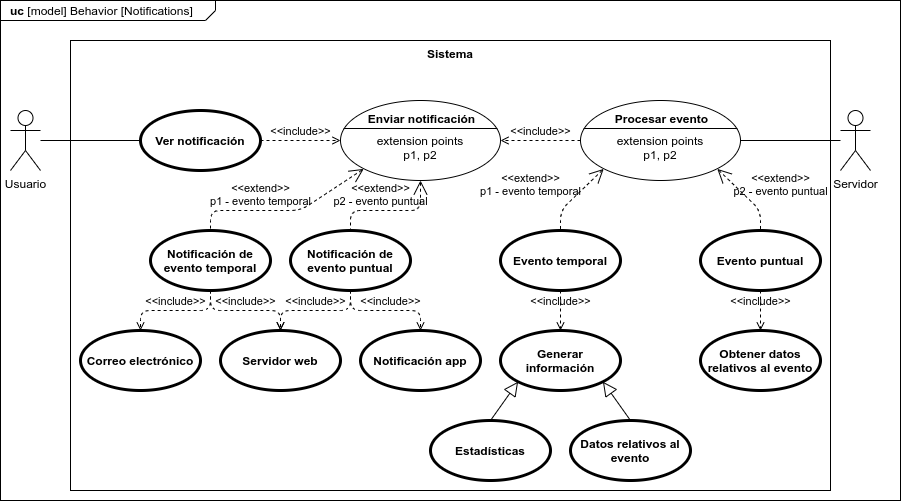
\includegraphics[width=\linewidth]{diagrams/UseCases-UC4 - notifications.png}
  \caption{Caso de uso \texttt{04} -- \textit{envío de notificaciones}.}
  \label{uc:notifications}
\end{figure}

\begin{table}[H]
  \centering
  \begin{tabularx}{\textwidth}{|c|c|X|}
    \hline
    \texttt{04}                                 & \multicolumn{2}{c|}{\textit{Envío de notificaciones}}                                                                                                                                                                                                                                                                                                                                                                                   \\
    \hline
    \textbf{Descripción}                        & \multicolumn{2}{X|}{El servidor, en conjunción con el resto de elementos del sistema, detecta ciertos eventos y actúa generando una notificación que envía al usuario.}                                                                                                                                                                                                                                                                 \\
    \hline
    \multirow{18}{*}{\textbf{Secuencia normal}} & \textbf{Paso}                                                                                                                                                           & \textbf{Acción}                                                                                                                                                                                                                                               \\
    \cline{2-3}
                                                & 1                                                                                                                                                                       & \multicolumn{1}{L|}{El servidor en un instante puntual produce y procesa un evento.}                                                                                                                                                                          \\
    \cline{2-3}
                                                & 1.1                                                                                                                                                                     & \multicolumn{1}{L|}{Si el evento se ha producido por un hecho (p.e.: repostar, finalizar un viaje, \dots), es un evento puntual sobre el cual se envía información relativa al mismo y al contexto (estadísticas del depósito, información del viaje, etc.).} \\
    \cline{2-3}
                                                & 1.2                                                                                                                                                                     & \multicolumn{1}{L|}{Si el evento se ha producido porque ha pasado un lapso de tiempo, es un evento temporal. El servidor generará estadísticas relativas a ese lapso de tiempo y mandará esa notificación.}                                                   \\
    \cline{2-3}
                                                & 2                                                                                                                                                                       & \multicolumn{1}{L|}{Se envía una notificación al usuario con los datos relativos al evento.}                                                                                                                                                                  \\
    \cline{2-3}
                                                & 2.1                                                                                                                                                                     & \multicolumn{1}{L|}{Si es un evento puntual, la notificación se envía a todos los medios: correo electrónico, servidor web y aplicación.}                                                                                                                     \\
    \cline{2-3}
                                                & 2.2                                                                                                                                                                     & \multicolumn{1}{L|}{Si es un evento temporal, la notificación se envía solo al correo electrónico y al servidor web.}                                                                                                                                         \\
    \cline{2-3}
                                                & 3                                                                                                                                                                       & \multicolumn{1}{L|}{El usuario recibe la notificación en alguno de los tres medios.}                                                                                                                                                                          \\
    \hline
  \end{tabularx}
\end{table}

\noindent\rule{\linewidth}{.2pt}

\begin{figure}[H]
  \centering
  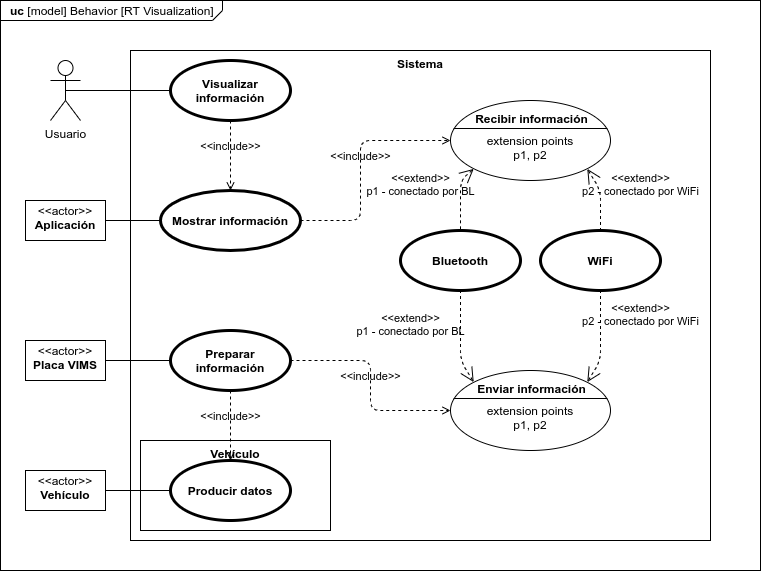
\includegraphics[width=\linewidth]{diagrams/UseCases-UC5 - visualization.png}
  \caption{Caso de uso \texttt{05} -- \textit{visualización en tiempo real}}
  \label{uc:visualization}
\end{figure}

\begin{table}[H]
  \centering
  \begin{tabularx}{\textwidth}{|c|c|X|}
    \hline
    \texttt{05}                                & \multicolumn{2}{c|}{\textit{Visualización en tiempo real}}                                                                                                                                                                                          \\
    \hline
    \textbf{Descripción}                       & \multicolumn{2}{X|}{Un usuario podrá visualizar información en tiempo real sobre su vehículo mediante la aplicación.}                                                                                                                               \\
    \hline
    \multirow{7}{*}{\textbf{Secuencia normal}} & \textbf{Paso}                                                                                                          & \textbf{Acción}                                                                                                            \\
    \cline{2-3}
                                               & 1                                                                                                                      & \multicolumn{1}{L|}{El usuario solicita visualizar información sobre el vehículo desde la aplicación.}                     \\
    \cline{2-3}
                                               & 2                                                                                                                      & \multicolumn{1}{L|}{La aplicación recibe la información de la placa \ac{VIMS} usando redes \ac{PAN}.}                      \\
    \cline{2-3}
                                               & 3                                                                                                                      & \multicolumn{1}{L|}{La placa \ac{VIMS} prepara la información que recibe del vehículo y la transmite hacia la aplicación.} \\
    \hline
    \multirow{10}{*}{\textbf{Excepciones}}     & \textbf{Paso}                                                                                                          & \textbf{Acción}                                                                                                            \\
    \cline{2-3}
                                               & 1.1                                                                                                                    & \multicolumn{1}{L|}{El usuario no está autenticado.}                                                                       \\
    \cline{2-3}
                                               & 1.2                                                                                                                    & \multicolumn{1}{L|}{El usuario no cuenta con ningún dispositivo \ac{VIMS} asociado.}                                       \\
    \cline{2-3}
                                               & 2.1                                                                                                                    & \multicolumn{1}{L|}{No hay conexión mediante Bluetooth, se realiza la comunicación por WiFi.}                              \\
    \cline{2-3}
                                               & 2.2                                                                                                                    & \multicolumn{1}{L|}{No hay conexión mediante WiFi, se realiza la comunicación por Bluetooth.}                              \\
    \cline{2-3}
                                               & 2.3                                                                                                                    & \multicolumn{1}{L|}{La placa \ac{VIMS} está desconectada.}                                                                 \\
    \cline{2-3}
                                               & 3                                                                                                                      & \multicolumn{1}{L|}{La placa \ac{VIMS} está desconectada o el vehículo no emite ningún dato.}                              \\
    \hline\hline
    \textbf{Resolución}                        & \multicolumn{2}{X|}{La placa no realiza ninguna transmisión de información hasta que no haya una conexión disponible.}                                                                                                                              \\
    \hline
  \end{tabularx}
\end{table}

\noindent\rule{\linewidth}{.2pt}

\begin{figure}[H]
  \centering
  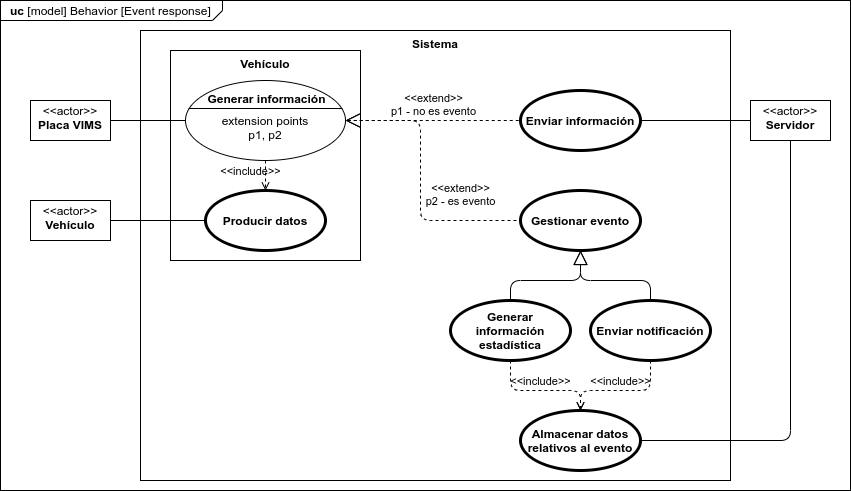
\includegraphics[width=\linewidth]{diagrams/UseCases-UC6 - reaction.png}
  \caption{Caso de uso \texttt{06} -- \textit{generación de eventos}}
  \label{uc:reaction}
\end{figure}

\begin{table}[H]
  \centering
  \begin{tabularx}{\textwidth}{|c|c|X|}
    \hline
    \texttt{06}                                 & \multicolumn{2}{c|}{\textit{Generación de eventos}}                                                                                                                                                                                                                                                                         \\
    \hline
    \textbf{Descripción}                        & \multicolumn{2}{X|}{El dispositivo \ac{VIMS}, a la hora de enviar datos, podrá producir eventos según el tipo de información que haya de enviar.}                                                                                                                                                                           \\
    \hline
    \multirow{10}{*}{\textbf{Secuencia normal}} & \textbf{Paso}                                                                                                                                     & \textbf{Acción}                                                                                                                                                         \\
    \cline{2-3}
                                                & 1                                                                                                                                                 & \multicolumn{1}{L|}{El dispositivo \ac{VIMS} genera información y la transmite hacia el servidor.}                                                                      \\
    \cline{2-3}
                                                & 1.1                                                                                                                                               & \multicolumn{1}{L|}{Si la información a transmitir es ``normal'', se envía directamente al servidor.}                                                                   \\
    \cline{2-3}
                                                & 1.2                                                                                                                                               & \multicolumn{1}{L|}{Si la información a transmitir es eventual, se procesa el evento generando información estadística referente al mismo o mandando una notificación.} \\
    \cline{2-3}
                                                & 2                                                                                                                                                 & \multicolumn{1}{L|}{El servidor recibe el evento y se encarga de gestionarlo, como se vio en el \texttt{UC-04}.}                                                        \\
    \hline
    \multirow{3}{*}{\textbf{Excepciones}}       & \textbf{Paso}                                                                                                                                     & \textbf{Acción}                                                                                                                                                         \\
    \cline{2-3}
                                                & 1                                                                                                                                                 & \multicolumn{1}{L|}{No hay ninguna cuenta asociada al dispositivo.}                                                                                                     \\
    \cline{2-3}
                                                & 1.1                                                                                                                                               & \multicolumn{1}{L|}{No hay conexión a Internet por parte del dispositivo \ac{VIMS}.}                                                                                    \\
    \hline\hline
    \textbf{Resolución}                         & \multicolumn{2}{X|}{La placa funciona en modo desconectado, es decir, no transmite datos al servidor.}                                                                                                                                                                                                                      \\
    \hline
  \end{tabularx}
\end{table}

\noindent\rule{\linewidth}{.2pt}

\begin{figure}[H]
  \centering
  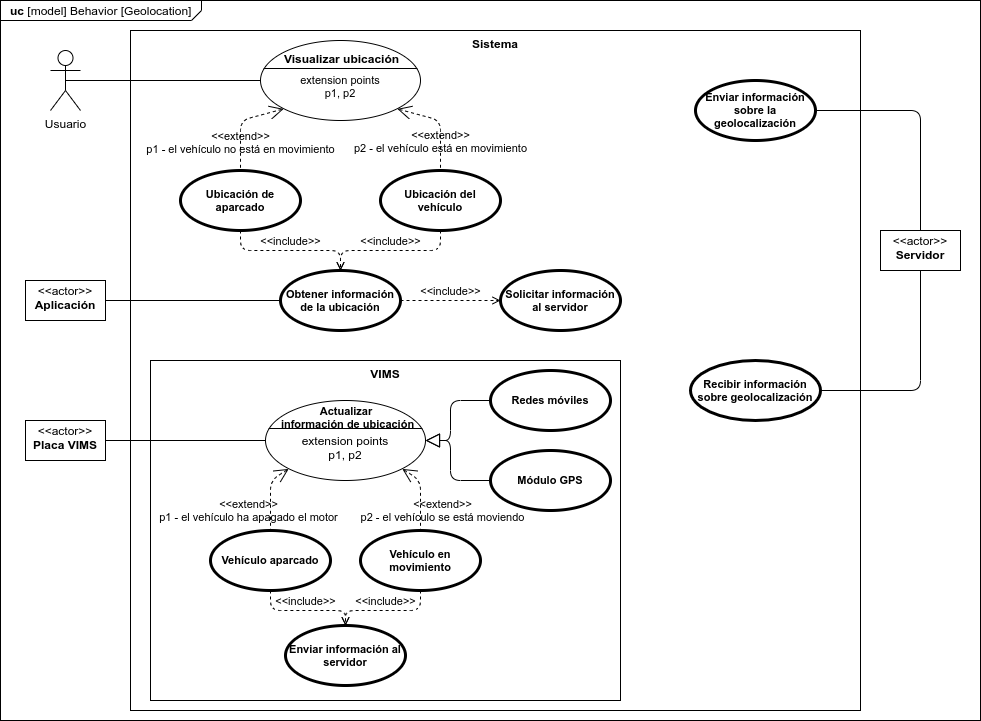
\includegraphics[width=\linewidth]{diagrams/UseCases-UC7 - location.png}
  \caption{Casos de uso \texttt{07*} -- \textit{envío, almacenamiento y visualización de geolocalización}}
  \label{uc:location}
\end{figure}

\begin{table}[H]
  \centering
  \begin{tabularx}{\textwidth}{|c|c|X|}
    \hline
    \texttt{07.1}                               & \multicolumn{2}{c|}{\textit{Visualización de ubicación}}                                                                                                                                                                                                                                                                                                        \\
    \hline
    \textbf{Descripción}                        & \multicolumn{2}{X|}{El usuario mediante una aplicación podrá visualizar la ubicación del vehículo en tiempo real. Si el vehículo está apagado, se visualiza la ubicación del aparcamiento.}                                                                                                                                                                     \\
    \hline
    \multirow{10}{*}{\textbf{Secuencia normal}} & \textbf{Paso}                                                                                                                                                                               & \textbf{Acción}                                                                                                                                                   \\
    \cline{2-3}
                                                & 1                                                                                                                                                                                           & \multicolumn{1}{L|}{El usuario inicia una aplicación para visualizar la ubicación de su vehículo.}                                                                \\
    \cline{2-3}
                                                & 1.1                                                                                                                                                                                         & \multicolumn{1}{L|}{Si el vehículo se encuentra en movimiento, se visualiza la ubicación en tiempo real según se va actualizando.}                                \\
    \cline{2-3}
                                                & 1.2                                                                                                                                                                                         & \multicolumn{1}{L|}{Si el vehículo está apagado se considera que está aparcado y se visualiza la última ubicación conocida, correspondiente con el aparcamiento.} \\
    \cline{2-3}
                                                & 2                                                                                                                                                                                           & \multicolumn{1}{L|}{Se realizan peticiones al servidor para obtener la información de la geolocalización.}                                                        \\
    \hline
    \multirow{3}{*}{\textbf{Excepciones}}       & \textbf{Paso}                                                                                                                                                                               & \textbf{Acción}                                                                                                                                                   \\
    \cline{2-3}
                                                & 1                                                                                                                                                                                           & \multicolumn{1}{L|}{No hay ningún dispositivo asociado a la cuenta.}                                                                                              \\
    \cline{2-3}
                                                & 1.1                                                                                                                                                                                         & \multicolumn{1}{L|}{El vehículo está desconectado de la red, por lo que no se pueden transmitir los datos de geolocalización.}                                    \\
    \cline{2-3}
                                                & 1.2                                                                                                                                                                                         & \multicolumn{1}{L|}{No hay ningún dato de geolocalización almacenado.}                                                                                            \\
    \cline{2-3}
                                                & 2                                                                                                                                                                                           & \multicolumn{1}{L|}{La aplicación no cuenta con conexión a la red.}                                                                                               \\
    \hline\hline
    \textbf{Resolución}                         & \multicolumn{2}{X|}{La placa funciona en modo desconectado, es decir, no transmite datos al servidor.}                                                                                                                                                                                                                                                          \\
    \hline
  \end{tabularx}
\end{table}

\begin{table}[H]
  \centering
  \begin{tabularx}{\textwidth}{|c|c|X|}
    \hline
    \texttt{07.2}                               & \multicolumn{2}{c|}{\textit{Envío de ubicación}}                                                                                                                                                                                                                                                 \\
    \hline
    \textbf{Descripción}                        & \multicolumn{2}{X|}{La placa \ac{VIMS} enviará la información relativa al vehículo al servidor.}                                                                                                                                                                                                 \\
    \hline
    \multirow{18}{*}{\textbf{Secuencia normal}} & \textbf{Paso}                                                                                    & \textbf{Acción}                                                                                                                                                                               \\
    \cline{2-3}
                                                & 1                                                                                                & \multicolumn{1}{L|}{La placa actualiza la información sobre la ubicación del vehículo.}                                                                                                       \\
    \cline{2-3}
                                                & 1.1                                                                                              & \multicolumn{1}{L|}{Si se ha perdido la conexión con el vehículo (motor apagado), se considera que está aparcado y se envía la ubicación actual como ``ubicación de aparcado''.}              \\
    \cline{2-3}
                                                & 1.2                                                                                              & \multicolumn{1}{L|}{Si el vehículo está activo (motor encendido), se considera que está en movimiento y envía de forma periódica la ubicación actual del vehículo.}                           \\
    \cline{2-3}
                                                & 2                                                                                                & \multicolumn{1}{L|}{Según la precisión de las redes y la disponibilidad de las mismas, la ubicación se obtiene mediante dos métodos.}                                                         \\
    \cline{2-3}
                                                & 2.1                                                                                              & \multicolumn{1}{L|}{Se obtiene la ubicación mediante el uso de redes móviles cuando el módulo GPS no se encuentre disponible o no se tengan suficientes satélites.}                           \\
    \cline{2-3}
                                                & 2.2                                                                                              & \multicolumn{1}{L|}{Se obtiene la ubicación mediante el módulo GPS como primera alternativa, y se usan las redes móviles cuando estén disponibles para mejorar la precisión de la ubicación.} \\
    \cline{2-3}
                                                & 3                                                                                                & \multicolumn{1}{L|}{Se manda la ubicación obtenida al servidor y se enlaza a la cuenta asociada.}                                                                                             \\
    \hline
    \multirow{6}{*}{\textbf{Excepciones}}       & \textbf{Paso}                                                                                    & \textbf{Acción}                                                                                                                                                                               \\
    \cline{2-3}
                                                & 1                                                                                                & \multicolumn{1}{L|}{No hay ninguna cuenta asociada al dispositivo.}                                                                                                                           \\
    \cline{2-3}
                                                & 1.1                                                                                              & \multicolumn{1}{L|}{No hay ninguna conectividad de red disponible para realizar el envío de la ubicación.}                                                                                    \\
    \cline{2-3}
                                                & 3                                                                                                & \multicolumn{1}{L|}{La conexión de red no está disponible para realizar la transmisión de la información.}                                                                                    \\
    \hline\hline
    \textbf{Resolución}                        & \multicolumn{2}{X|}{La placa funciona en modo desconectado, es decir, no transmite datos al servidor.}                                                                                                                                                      \\
    \hline
  \end{tabularx}
\end{table}

\begin{table}[H]
  \centering
  \begin{tabularx}{\textwidth}{|c|c|X|}
    \hline
    \texttt{07.3}                              & \multicolumn{2}{c|}{\textit{Almacenamiento de los datos de ubicación}}                                                                                                                                                                                                        \\
    \hline
    \textbf{Descripción}                       & \multicolumn{2}{X|}{El servidor almacenará y gestionará los datos de ubicación recibidos por los múltiples dispositivos \ac{VIMS}.}                                                                                                                                           \\
    \hline
    \multirow{8}{*}{\textbf{Secuencia normal}} & \textbf{Paso}                                                                                                                       & \textbf{Acción}                                                                                                                         \\
    \cline{2-3}
                                               & 1                                                                                                                                   & \multicolumn{1}{L|}{El servidor recibe la información de la ubicación de un dispositivo \ac{VIMS}.}                                     \\
    \cline{2-3}
                                               & 1.1                                                                                                                                 & \multicolumn{1}{L|}{Los datos de ubicación se almacenan en una línea temporal para poder ver el histórico de ubicaciones del vehículo.} \\
    \cline{2-3}
                                               & 1.2                                                                                                                                 & \multicolumn{1}{L|}{El último valor de ubicación se almacena para una posterior visualización.}                                         \\
    \cline{2-3}
                                               & 2                                                                                                                                   & \multicolumn{1}{L|}{El servidor ofrece los datos de ubicación a través de la \ac{API}.}                                                 \\
    \hline
    \multirow{2}{*}{\textbf{Excepciones}}      & \textbf{Paso}                                                                                                                       & \textbf{Acción}                                                                                                                         \\
    \cline{2-3}
                                               & 1                                                                                                                                   & \multicolumn{1}{L|}{No hay ninguna cuenta asociada al dispositivo.}                                                                     \\
    \hline\hline
    \textbf{Resolución}                        & \multicolumn{2}{X|}{La placa funciona en modo desconectado, es decir, no transmite datos al servidor.}                                                                                                                                                      \\
    \hline
  \end{tabularx}
\end{table}

\section{Diagramas de bloques}
\begin{figure}[H]
  \centering
  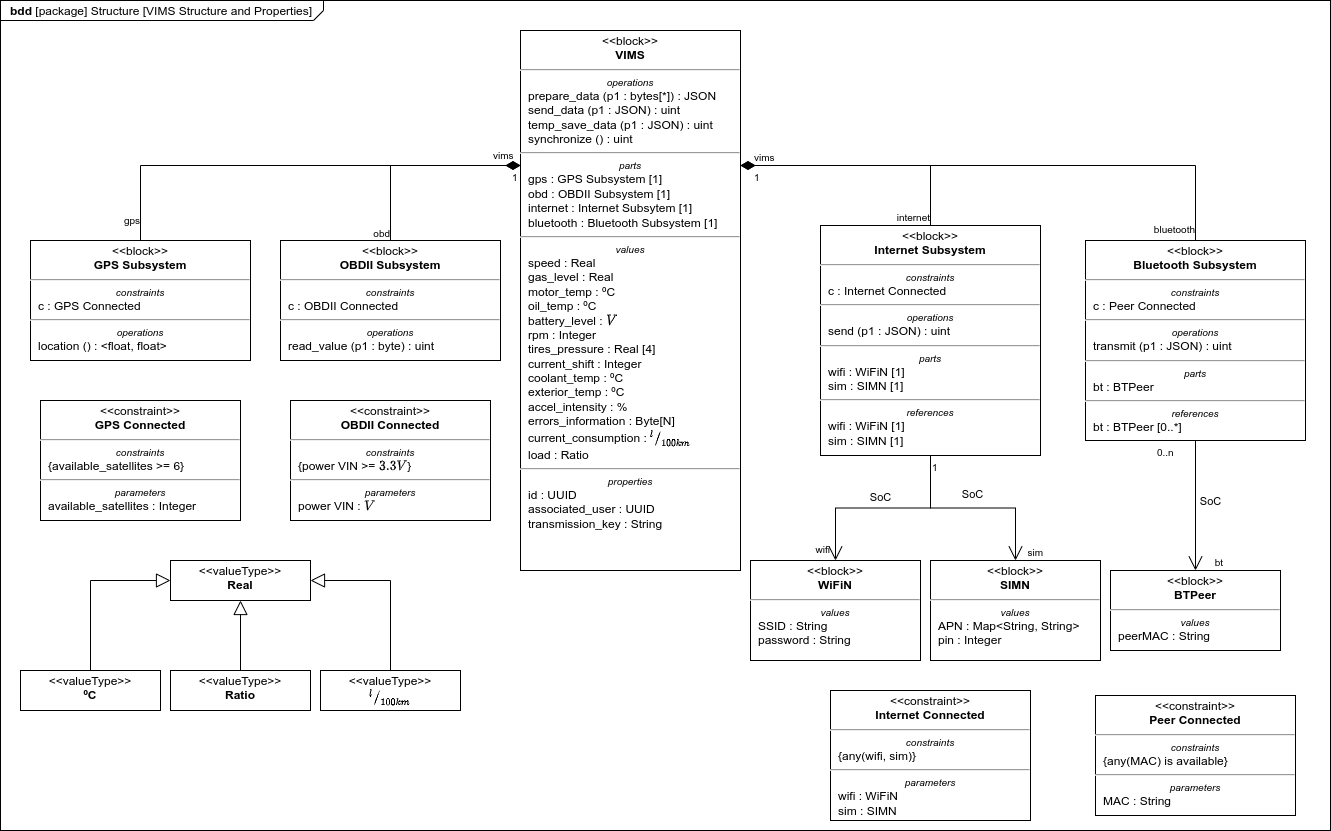
\includegraphics[width=\linewidth]{images/BlockDiagrams-VIMS.drawio.png}
  \caption{Diagrama de bloques que modela el conjunto de la placa \ac{VIMS} y sus componentes.}
  \label{bd:vims}
\end{figure}

\begin{figure}[H]
  \centering
  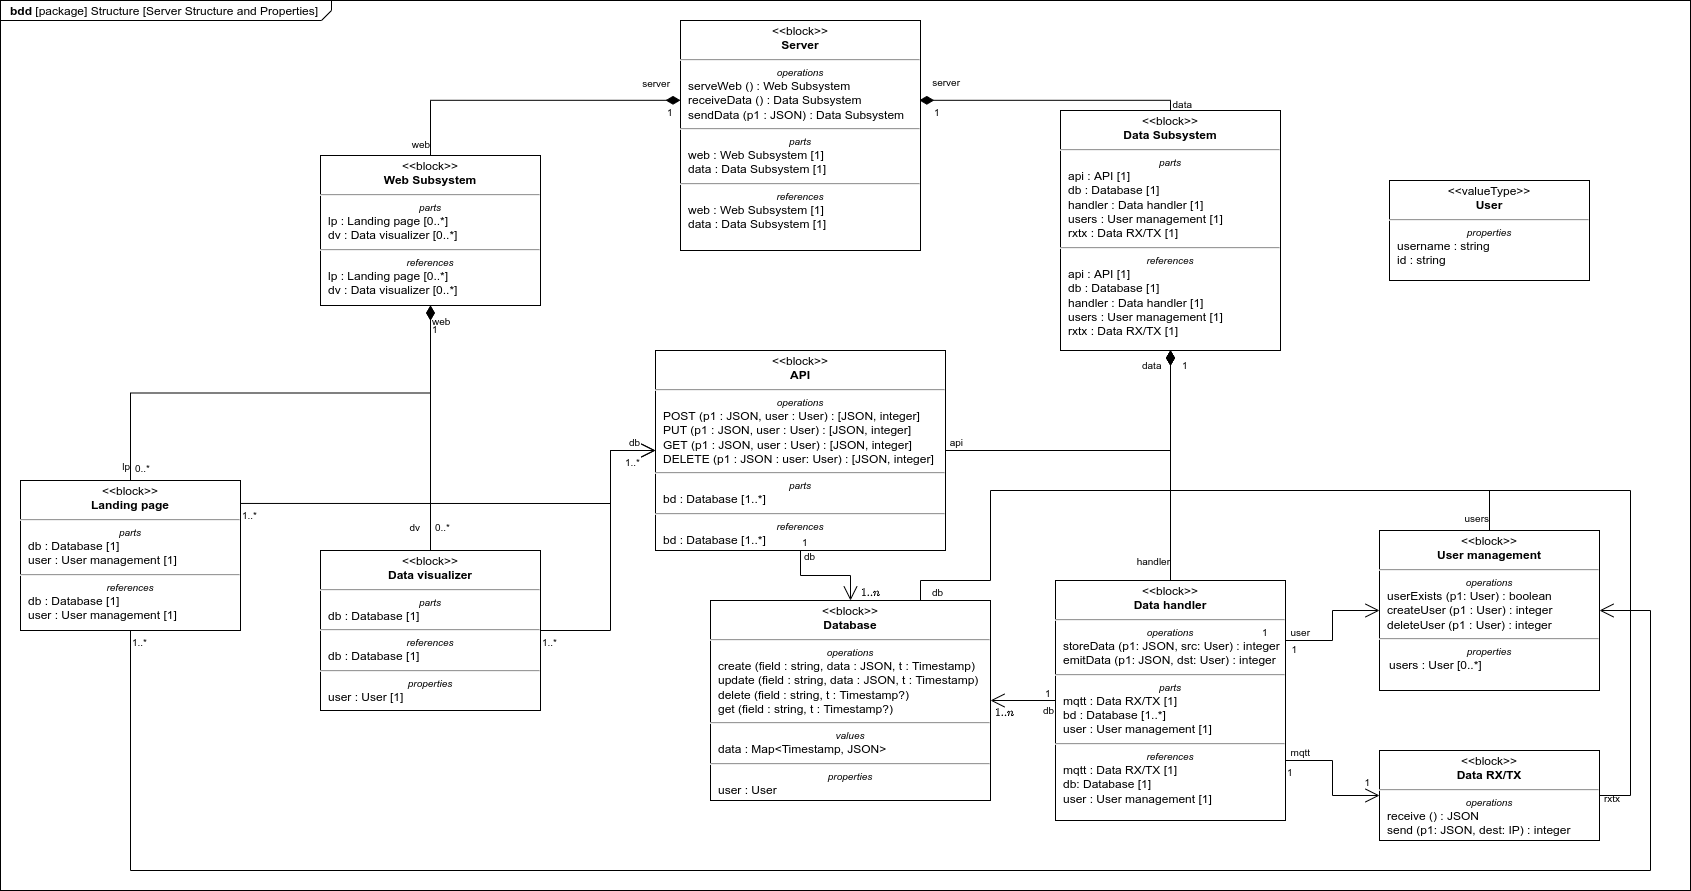
\includegraphics[width=\linewidth]{images/BlockDiagrams-Server.drawio.png}
  \caption{Diagrama de bloques que modela al servidor y sus components.}
  \label{bd:server}
\end{figure}

\begin{figure}[H]
  \centering
  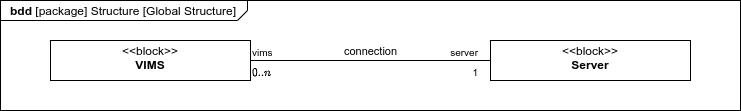
\includegraphics[width=\linewidth]{images/BlockDiagrams-Global.drawio.png}
  \caption{Diagrama global del sistema. Como se puede ver, se sigue una arquitectura cliente--servidor.}
  \label{bd:global}
\end{figure}
